\resizebox{\textwidth}{!}{%
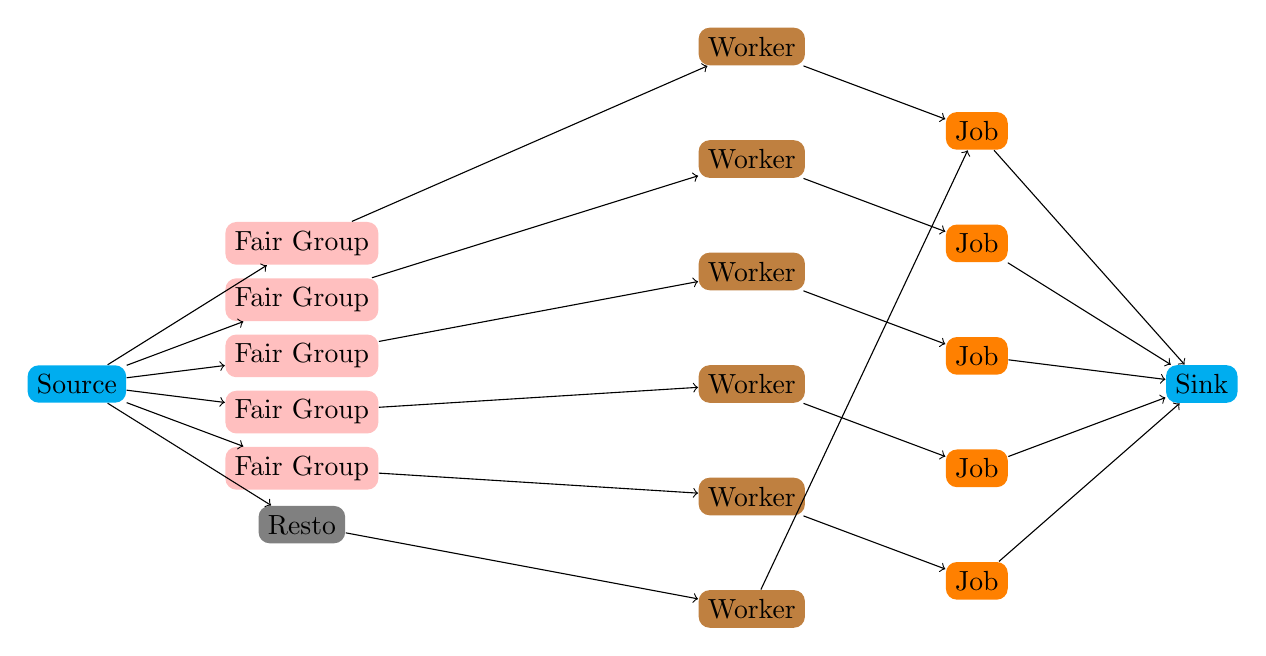
\begin{tikzpicture}
    % Define the nodes
    \node[fill=cyan, rounded corners] (source) at (-7.5, 0.0) {Source};
    \node[fill=pink, rounded corners] (group1) at (-4.643, 1.786) {Fair Group};
    \node[fill=pink, rounded corners] (group2) at (-4.643, 1.071) {Fair Group};
    \node[fill=pink, rounded corners] (group3) at (-4.643, 0.357) {Fair Group};
    \node[fill=pink, rounded corners] (group4) at (-4.643, -0.357) {Fair Group};
    \node[fill=pink, rounded corners] (group5) at (-4.643, -1.071) {Fair Group};
    \node[fill=gray, rounded corners] (resto) at (-4.643, -1.786) {Resto};
    
    \node[fill=brown, rounded corners] (worker1) at (1.071, 4.286) {Worker};
    \node[fill=brown, rounded corners] (worker2) at (1.071, 2.857) {Worker};
    \node[fill=brown, rounded corners] (worker3) at (1.071, 1.429) {Worker};
    \node[fill=brown, rounded corners] (worker4) at (1.071, 0.0) {Worker};
    \node[fill=brown, rounded corners] (worker5) at (1.071, -1.429) {Worker};
    \node[fill=brown, rounded corners] (worker6) at (1.071, -2.857) {Worker};
    
    \node[fill=orange, rounded corners] (job1) at (3.929, 3.214) {Job};
    \node[fill=orange, rounded corners] (job2) at (3.929, 1.786) {Job};
    \node[fill=orange, rounded corners] (job3) at (3.929, 0.357) {Job};
    \node[fill=orange, rounded corners] (job4) at (3.929, -1.071) {Job};
    \node[fill=orange, rounded corners] (job5) at (3.929, -2.5) {Job};
    
    \node[fill=cyan, rounded corners] (target) at (6.786, 0.0) {Sink};
    
    % Draw the edges
    \draw[->] (source) -- (group1);
    \draw[->] (source) -- (group2);
    \draw[->] (source) -- (group3);
    \draw[->] (source) -- (group4);
    \draw[->] (source) -- (group5);
    \draw[->] (source) -- (resto);
    
    \draw[->] (group1) -- (worker1);
    \draw[->] (group2) -- (worker2);
    \draw[->] (group3) -- (worker3);
    \draw[->] (group4) -- (worker4);
    \draw[->] (group5) -- (worker5);
    \draw[->] (resto) -- (worker6);
    
    \draw[->] (worker1) -- (job1);
    \draw[->] (worker2) -- (job2);
    \draw[->] (worker3) -- (job3);
    \draw[->] (worker4) -- (job4);
    \draw[->] (worker5) -- (job5);
    \draw[->] (worker6) -- (job1);
    
    \draw[->] (job1) -- (target);
    \draw[->] (job2) -- (target);
    \draw[->] (job3) -- (target);
    \draw[->] (job4) -- (target);
    \draw[->] (job5) -- (target);
\end{tikzpicture}
}%
